\documentclass[
    english, spanish, Ce-table, Ce-theorem
]{CabesHW}
\usepackage[utf8]{inputenc}
\usepackage{parskip}
\usepackage[es-tabla]{babel}
\usepackage{hyperref}
\usepackage{algpseudocodex}
\usepackage{minted}
\usepackage{siunitx}

%%%%%%%%%%%%%%%%%%%%%%%%%%%%%%%%%
%% Configuraciones adicionales %%
%%%%%%%%%%%%%%%%%%%%%%%%%%%%%%%%%
\makeatletter

%% Algpseudocodex restyling %%
\renewcommand{\algpx@commentFormat}[1]{%
	\ifbool{algpx@italicComments}{%
		\textsl{\textcolor{\algpx@commentColor}{#1}}%
	}{%
		\textcolor{\algpx@commentColor}{#1}%
	}%
}

%% myalg environment %%
\newenvironment{myalg}{%algorithm
    \begin{minipage}{0.8\textwidth}
    \selectlanguage{english}
    \begin{algorithmic}%
}{%
    \end{algorithmic}
    \end{minipage}%
}

%% Float new environments %%
\newfloat{algorithm}{tbp}{loa}
\floatname{algorithm}{Algoritmo}

\makeatother
\endinput
\decimalpoint
\usemintedstyle{lovelace}
\hypersetup{
    colorlinks=true,
    allcolors=blue!65!black
}

\institute{Escuela de Ciencias Físicas y Matemática}
\title{Proyecto 4}
\author{Amado Cabrera, Denilson Mendoza y Mariana Pérez}
\id{201905757, 202005724 y 201901040}
\date{\today}
\course{Laboratorio de simulación}
\professor{Carlos Soto}

\begin{document}

\maketitle

\begin{abstract}
Este proyecto de clase consistió en aplicar y comparar tres métodos numéricos para resolver ecuaciones diferenciales ordinarias: Euler, Taylor y Runge--Kutta, siendo estos dos últimos de cuarto orden. El objetivo de este proyecto era analizar el rendimiento de estos métodos al comparar su precisión. Para cada método, se escribió un programa en C para calcular el valor de una ecuación de crecimiento poblacional. A continuación, los programas fueron probados y comparados. El método de Euler, que es un método de primer orden, resultó ser el menos preciso y eficiente de los tres métodos. El método de Taylor, que es un método de orden superior, era más preciso pero es más complejo de calcular. Por último, el método Runge--Kutta, que es un método de cuarto orden, resultó ser el más preciso y eficaz de los tres.
\end{abstract}

\vspace{0.5em}
\section{Marco teórico}
\subsection{Método de Euler}
El método de Euler permite obtener aproximaciones $w_i \approx y_{(x_i)}$ al problema de valor inicial bien planteado
\begin{align*}
\label{1.1}
    \td{y}{t} = f_{(x,y)}, \qquad a \leq t \leq b, \qquad y_{(a)} = \alpha. \tag{1.1}
\end{align*}

Este método no brinda una aproximación continua a la solución $y_{(x)}$, sino que genera aproximaciones de $y_{(x)}$ para varios valores de $x$ en el intervalo $[a, b]$. Dichos valores, denotados como $x_i$ y llamados \textit{puntos de malla}, deben estar distribuidos equitativamente en el intervalo. Para ello, se toma un número entero positivo $N$ (que representa la cantidad de pasos en el intervalo) y se seleccionan los puntos de malla
\[ x_i = a + ih, \qquad \text{para cada $i = 0, 1, \ldots, N$}; \]
donde $h = (b-a)/N = x_{i+1} - x_i$ es la distancia que existe entre cada $x_i$, por lo que $h$ recibe el nombre de \textit{tamaño del paso}.

Se usará el teorema de Taylor para derivar el método de Euler. Suponer que la solución de la ecuación  \eqref{1.1} tiene dos derivadas continuas en el intervalo $[a, b]$, por lo que para cada $i = 0, 1, \ldots, N-1$
\begin{align*}
     y_{(x)} &= y_{x_i} + (x-x_i)y'_{(x_i)} + \frac{(x-x_i)^2}{2!}y''_{(\xi_i)}.
\end{align*} 
Valuando la expresión en $x=x_{i+1}$:
\begin{align*}
     y_{(x_{i+1})} &= y_{x_i} + (x_{i+1}-x_i)y'_{(x_i)} + \frac{(x_{i+1}-x_i)^2}{2!}y''_{(\xi_i)}\\
     &= y_{x_i} + hy'_{(x_i)} + \frac{h^2}{2!}y''_{(\xi_i)}.
\end{align*}
El método de Euler se consigue descartando el término restante que incluye $\xi_i$:
\begin{align*}
    w_0 &= \alpha,\\
    w_{i+1} &= w_i + h f_{(t_i, w_i)}, \qquad \text{para cada $i = 0, 1, \ldots, N-1$}.
\end{align*}

\subsubsection{Pseudo--código}
\begin{algorithm}[H]
    \centering
    \begin{myalg}[1]
    \LComment{Método de Euler para resolución numérica de EDO}
    \Function{Edo}{$x$, $y$}
        \State \Output $0.16 y$
    \EndFunction
    \State \phantom{}
    \State $x_i \gets 0$ \Comment{Valor inicial de $x$}
    \State $y_i \gets 367$ \Comment{Valor inicial de $y$}
    \State $x_f \gets 20$ \Comment{Valor final de $x$}
    \State $n \gets 100$ \Comment{Número máximo de pasos}
    \State \phantom{}
    \State $h \gets (x_f - x_i)/n$ \Comment{Valor del paso}
    \For{$i = 0,\ldots,n$}
        \State \Output $(i, x_i, y_i)$
        \State \phantom{}
        \State $y_i \gets y_i + h\cdot\Call{Edo}{x_i, y_i}$
        \State $x_i \gets x_i + h$
    \EndFor
    \end{myalg}
    \caption{Pseudo--código para el método de Euler.}
    \label{alg:euler}
\end{algorithm}

\vspace{1em}
\subsection{Método de Taylor}
Suponer que la solución a la ecuación
\[ \td{y}{x} = f_{(x,y)}, \qquad a \leq t \leq b, \qquad y_{(a)} = \alpha \]
tiene $n+1$ derivadas continuas.

Derivando repetidas veces la solución se obtiene
\begin{align*}
\label{tay2.1}
    y^{(k)}_{(x)} &= f^{(k-1)}_{(x, y_{(x)})}. \tag{2.1}
\end{align*}

Empleando el $n$-ésimo polinomio de Taylor al rededor de $x_i$, expandir la solución $y_{(x)}$ y posteriormente valuarla en $x= x_{i+1}$:
\begin{align*}
    y_{(x)} &= y_{x_i} + (x-x_i)y'_{(x_i)} + \frac{(x-x_i)^2}{2!}y''_{(x_i)} + \ldots + \frac{(x-x_i)^{n}}{n!}y^{(n)}_{(x_i)} + \frac{(t-x_i)^{n+1}}{(n+1)!}y^{(n+1)}_{(\xi_i)}\\
    y_{(x_{i+1})} &= y_{x_i} + (x_{i+1}-x_i)y'_{(x_i)} + \frac{(x_{i+1}-x_i)^2}{2!}y''_{(x_i)} + \ldots + \frac{(x_{i+1}-x_i)^{n}}{n!}y^{(n)}_{(\xi_i)} + \frac{(x_{i+1}-x_i)^{n+1}}{(n+1)!}y^{(n+1)}_{(x_i)}\\
\label{tay2.2}
    y_{(x_{i+1})} &= y_{x_i} + hy'_{(x_i)} + \frac{h^2}{2!}y''_{(x_i)} + \ldots + \frac{h^{n}}{n!}y^{(n)}_{(x_i)} + \frac{h^{n+1}}{(n+1)!}y^{(n+1)}_{(\xi_i)}, \tag{2.2}
\end{align*}
para algún $\xi_i$ en $(x_i, x_{i+1})$.

Reemplazando \eqref{tay2.1} en \eqref{tay2.2}, se consigue
\begin{align*}
    y_{(x_{i+1})} &= y_{x_i} + hf_{(x_i, y_{(x_i)})} + \frac{h^2}{2!}f'_{(x_i, y_{(x_i)})} + \ldots + \frac{h^{n}}{n!}f^{(n-1)}_{(x_i, y_{(x_i)})} + \frac{h^{n+1}}{(n+1)!}f^{(n)}_{(\xi_i, y_{(\xi_i)})}
\end{align*}

El método de Taylor de orden $n$ se consigue descartando el término restante que incluye $\xi_i$:
\begin{align*}
    w_0 &= \alpha,\\
    w_{i+1} &= w_i + hT^{(n)}_{(x_i, w_i)}, \qquad \text{para cada $i = 0, 1, \ldots, N-1$};
\end{align*}
donde
\begin{align*}
    T^{(n)}_{(x_i, w_i)} &= f_{(x_i, y_{(x_i)})} + \frac{h}{2!}f'_{(x_i, y_{(x_i)})} + \ldots + \frac{h^{n-1}}{n!}f^{(n-1)}_{(x_i, y_{(x_i)})} .
\end{align*}

\subsubsection{Pseudo--código}
\begin{algorithm}[H]
    \centering
    \begin{myalg}[1]
    \LComment{Método de Taylor para resolución numérica de EDO}
    \Function{Edo}{$x$, $y$} \Comment{Edo y sus derivadas}
        \State \Output $0.16 y$
    \EndFunction
    \State \phantom{}
    \Function{dEdo}{$x$, $y$} \Comment{Derivada 1}
        \State \Output $0.16 \Call{Edo}{x,y}$
    \EndFunction
    \State \phantom{}
    \Function{ddEdo}{$x$, $y$} \Comment{Derivada 2}
        \State \Output $0.16 \Call{dEdo}{x,y}$
    \EndFunction
    \State \phantom{}
    \Function{dddEdo}{$x$, $y$} \Comment{Derivada 3}
        \State \Output $0.16 \Call{ddEdo}{x,y}$
    \EndFunction
    \State \phantom{}
    \State $x_i \gets 0$ \Comment{Valor inicial de $x$}
    \State $y_i \gets 367$ \Comment{Valor inicial de $y$}
    \State $x_f \gets 20$ \Comment{Valor final de $x$}
    \State $n \gets 100$ \Comment{Número máximo de pasos}
    \State \phantom{}
    \State $h \gets (x_f - x_i)/n$ \Comment{Valor del paso}
    \For{$i = 0,\ldots,n$}
        \State \Output $(i, x_i, y_i)$
        \State \phantom{}
        \State $y_i \gets y_i + h(\Call{Edo}{x_i, y_i} + h\cdot\Call{dEdo}{x_i, y_i}/2 + $
        \Statex \hspace{5em}$+ h^2\cdot\Call{ddEdo}{x_i, y_i}/6 + h^3\cdot\Call{dddEdo}{x_i, y_i}/24)$
        \State $x_i \gets x_i + h$
    \EndFor
    \end{myalg}
    \caption{Pseudo--código para el método de Taylor.}
    \label{alg:taylor}
\end{algorithm}

\vspace{1em}
\subsection{Método de Runge--Kutta}
Los métodos de Runge-Kutta tienen el error de truncamiento local de alto orden de los métodos de Taylor, pero eliminan la necesidad de calcular y evaluar las derivadas de $f_{(t, y)}$.

El método de Runge--Kutta de orden $n$ se deriva a partir de aproximar
\begin{align*}
    T^{(n)}_{(x_i, w_i)} &= f_{(x_i, y_{(x_i)})} + \frac{h}{2!}f'_{(x_i, y_{(x_i)})} + \ldots + \frac{h^{n-1}}{n!}f^{(n-1)}_{(x_i, y_{(x_i)})}. 
\end{align*}


El método de Runge--Kutta de cuarto orden es el método más utilizado y está dado por:
\begin{align*}
    w_0 &= \alpha,\\
    w_{i+1} &= w_i + \frac{1}{6}(k_1 + 2k_2 + 2k_3 + k_4), \qquad \text{para cada $i= 0, 1, \ldots, N-1$;}
\end{align*}
donde
\begin{align*}
    k_1 &= hf_{(x_i, w_i)},\\
    k_2 &= hf_{(x_i + \frac{h}{2}, w_i + \frac{1}{2}k_1)},\\
    k_3 &= hf_{(x_i + \frac{h}{2}, w_i + \frac{1}{2}k_2)},\\
    k_4 &= hf_{(x_{i+1}, w_i + k_3)}.
\end{align*}

\subsubsection{Pseudo--código}
\begin{algorithm}[H]
    \centering
    \begin{myalg}[1]
    \LComment{Método de Runge--Kutta para resolución numérica de EDO}
    \Function{Edo}{$x$, $y$}
        \State \Output $0.16 y$
    \EndFunction
    \State \phantom{}
    \State $x_i \gets 0$ \Comment{Valor inicial de $x$}
    \State $y_i \gets 367$ \Comment{Valor inicial de $y$}
    \State $x_f \gets 20$ \Comment{Valor final de $x$}
    \State $n \gets 100$ \Comment{Número máximo de pasos}
    \State \phantom{}
    \State $h \gets (x_f - x_i)/n$ \Comment{Valor del paso}
    \For{$i = 0,\ldots,n$}
        \State \Output $(i, x_i, y_i)$
        \State \phantom{}
        \State $k_1 \gets h\cdot\Call{Edo}{x_i, y_i}$
        \State $k_2 \gets h\cdot\Call{Edo}{x_i+h/2, y_i+k_1/2}$
        \State $k_3 \gets h\cdot\Call{Edo}{x_i+h/2, y_i+k_2/2}$
        \State $k_4 \gets h\cdot\Call{Edo}{x_i+h, y_i+k_3}$
        \State \phantom{}
        \State $y_i \gets y_i + h(k_1 + 2k_2 + 2k_3 + k_4)/6$
        \State $x_i \gets x_i + h$
    \EndFor
    \end{myalg}
    \caption{Pseudo--código para el método de Runge--Kutta.}
    \label{alg:runge-kutta}
\end{algorithm}

\section{Resultados}
\subsection{Tabulación de datos obtenidos}
\begin{table}[H]
    \centering
    \begin{tabular}{c|ccc}
    $i$ & $x_i$ & $y_i$ & $\varepsilon_i$\\[.1em]
    \hline\\[-.9em]
    \input{|python3 data/tabulardatos.py "data/data-eulerEr.csv"}
    \end{tabular}
    \caption{Datos obtenidos por el método de Euler.}
    \label{tab:euler}
\end{table}

\begin{table}[H]
    \centering
    \begin{tabular}{c|ccc}
    $i$ & $x_i$ & $y_i$ & $\varepsilon_i$\\[.1em]
    \hline\\[-.9em]
    \input{|python3 data/tabulardatos.py "data/data-taylorEr.csv"}
    \end{tabular}
    \caption{Datos obtenidos por el método de Taylor de cuarto orden.}
    \label{tab:taylor}
\end{table}

\begin{table}[H]
    \centering
    \begin{tabular}{c|ccc}
    $i$ & $x_i$ & $y_i$ & $\varepsilon_i$\\[.1em]
    \hline\\[-.9em]
    \input{|python3 data/tabulardatos.py "data/data-rungekuttaEr.csv"}
    \end{tabular}
    \caption{Datos obtenidos por el método de Runge--Kutta de cuarto orden.}
    \label{tab:runge-kutta}
\end{table}

\vspace{2em}
\subsection[Gráficas del error]{Gráficas del error $\boldsymbol{\varepsilon_{(x_i)}}$}
\begin{figure}[H]
    \centering
    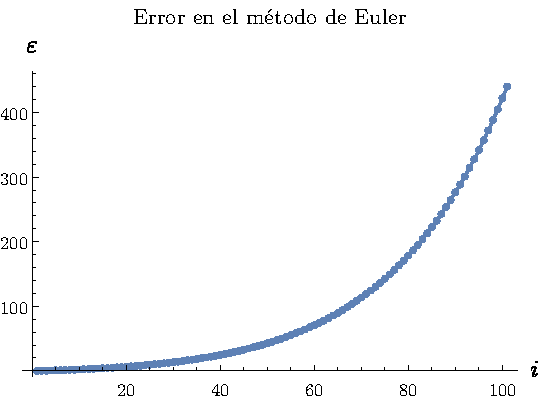
\includegraphics{imgs/plot-euler.pdf}
    \caption{Gráfica del error para el método de Euler.}
    \label{fig:euler}
\end{figure}

\begin{figure}[H]
    \centering
    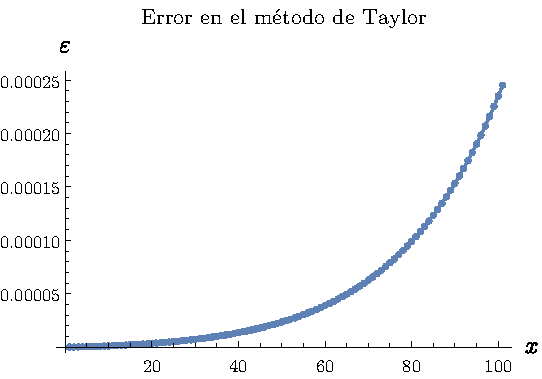
\includegraphics{imgs/plot-taylor.pdf}
    \caption{Gráfica del error para el método de Taylor de cuarto orden.}
    \label{fig:taylor}
\end{figure}

\begin{figure}[H]
    \centering
    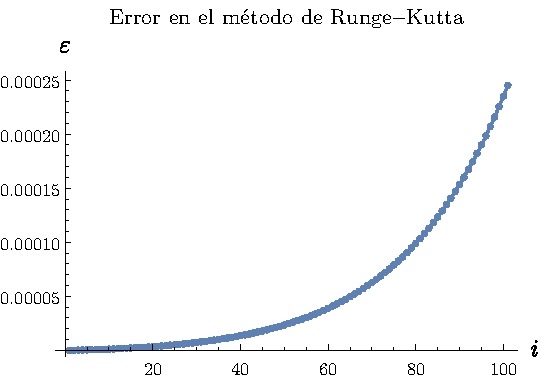
\includegraphics{imgs/plot-runge_kutta.pdf}
    \caption{Gráfica del error para el método de Runge--Kutta.}
    \label{fig:runge_kutta}
\end{figure}

\end{document}
